\documentclass[11pt]{article}
\usepackage[final]{acl}
\usepackage{times}
\usepackage{latexsym}
\usepackage[T1]{fontenc}
\usepackage[utf8]{inputenc}
\usepackage{microtype}
\usepackage{inconsolata}
\usepackage{graphicx}
\usepackage{booktabs}
\usepackage{multirow}
\usepackage{array}
\graphicspath{{figures/}}

\title{Making Tool Choice Observable: A Receipt-Safe Diagnostic Study of VOI-Based Memory in a Toolized Text Environment}

\author{Bochuan Yao\\
Boston University, CS505: Natural Language Processing\\
\texttt{yaobc@bu.edu}}

\begin{document}
\maketitle

\begin{abstract}
Tool-using language agents must often decide whether to act immediately or pay for information that may improve a later action. In multi-tool settings, this splits into two questions: whether to ask and which tool family to ask. This report extends the midway study of \texttt{voi\_memory\_v1}, a family-scoped memory variant tested in a cloneable ToyTextMDP environment with \textsc{scan}, \textsc{verify}, and \textsc{choose} actions. Since the midway report, I added scaled dual-battery runs, repaired reference generation, stricter receipt checks, and a v4 aggressive-stress task ecology designed to expose scan/verify conflict. The final receipt-safe v4 seed-7 battery does not support a stable which-tool improvement: choose-swallow and family-mismatch rates slightly worsen from reference to stress under the locked \texttt{voi\_memory\_v1} comparison, and verify usage drops. Both blocked-step audits point to task pressure rather than a localized gate, memory, or selector failure. The result is a negative one, but it is informative because the framework makes the tool-choice claim observable and then rejects it under controlled conditions.
\end{abstract}

\section{Introduction}

Language agents are increasingly evaluated as systems that reason, call tools, receive observations, and revise behavior over time \citep{karpas2022mrkl,mialon2023augmented,yao2023react,schick2023toolformer,qin2024toolllm,shinn2023reflexion,liu2024agentbench,jimenez2024swebench}. A central decision in these systems is epistemic: should the agent act now, or should it ask for more information? In a multi-tool setting, there is a second layer. If asking is useful, which information source should be queried?

The midway report narrowed the original broad proposal into a controlled diagnostic problem. It asked whether a family-scoped memory variant, \texttt{voi\_memory\_v1}, could make a meaningful which-tool problem observable in a small, cloneable text environment. The 10-task smoke batch exposed nonzero tool-choice opportunity, but tool precision stayed at ceiling and blocked \texttt{voi\_memory\_v1} rows still pointed to task pressure. At that point, the evidence supported whether-to-ask progress only.

The final experiments add the missing larger batteries and confirmation checks. I ran receipt-safe dual batteries, repaired reference packs when preflight failed, and tested a stronger v4 stress ecology. The result is stable but negative: under the current task profiles, \texttt{voi\_memory\_v1} does not improve the locked which-tool comparison. The value of the study is that a broad agent-memory claim becomes a concrete comparison that can fail.

The paper makes three contributions. First, it defines the task and memory machinery precisely enough for a classmate to inspect it. Second, it reports the post-midway evaluation sequence, separating offline diagnostics from receipt-safe live evidence. Third, it shows that the current bottleneck is best explained by task pressure rather than by evidence that the gate, memory, or selector should be edited.

The final report is organized around two research questions. RQ1 asks whether the stronger post-midway task ecologies expose enough live scan/verify conflict for a which-tool comparison to be meaningful. RQ2 asks whether \texttt{voi\_memory\_v1}, once evaluated only through receipt-safe batteries, improves that comparison. The answer to RQ1 is yes in a limited diagnostic sense: the v4 stress pack exposes wrong-tool surface in non-memory modes. The answer to RQ2 is no: the locked memory mode does not improve the final reference/stress comparison.

\section{Method}

\paragraph{Environment.}
ToyTextMDP is a finite-horizon text decision environment in the reinforcement-learning sense \citep{sutton2018reinforcement}. At each state $x_t$, the agent sees a hidden-answer task through text. It may choose immediately with \textsc{choose} actions, or pay a small cost for information using \textsc{scan} or \textsc{verify}. \textsc{scan} is cheaper but can be ambiguous; \textsc{verify} is more reliable and is sometimes necessary under the active task profiles. The environment supports exact cloning, so candidate action sequences can be evaluated in deterministic successor states.

\paragraph{Example step.}
In one v4 stress task, the hidden answer is A. The visible candidates include direct \textsc{choose\_a}, a cheap \textsc{scan} clue that supports A at cost .02, and a higher-reliability \textsc{verify} clue that also supports A at cost .05. The live \texttt{voi\_memory\_v1} policy chooses A immediately and receives reward, but oracle replay scores the best tool action as \textsc{scan} (.98) over \textsc{verify} (.95). This row is therefore a task success but a tool-choice failure: it enters the tool-opportunity denominator and is counted as choose-swallow.

\paragraph{Agent pipeline.}
The agent first generates candidate plans, filters ask candidates, scores the remaining candidates, and executes one action. The expanded decision equation is:
\[
\begin{array}{rcl}
C_t & = & \mathrm{Gen}(x_t, M_t) \\
\tilde{C}_t & = & \mathrm{Gate}(C_t, x_t, M_t) \\
a_t & = & \mathrm{Select}(\tilde{C}_t).
\end{array}
\]
Here $C_t$ is the candidate set, $M_t$ is retrieved memory, and $a_t$ is the selected action. The gate is not a general selector. It only decides whether \textsc{ask} candidates remain eligible before final arbitration. The selector then compares direct choice, scan plans, and verify plans using counterfactual scores plus structured penalties.

\begin{figure*}[t]
\centering
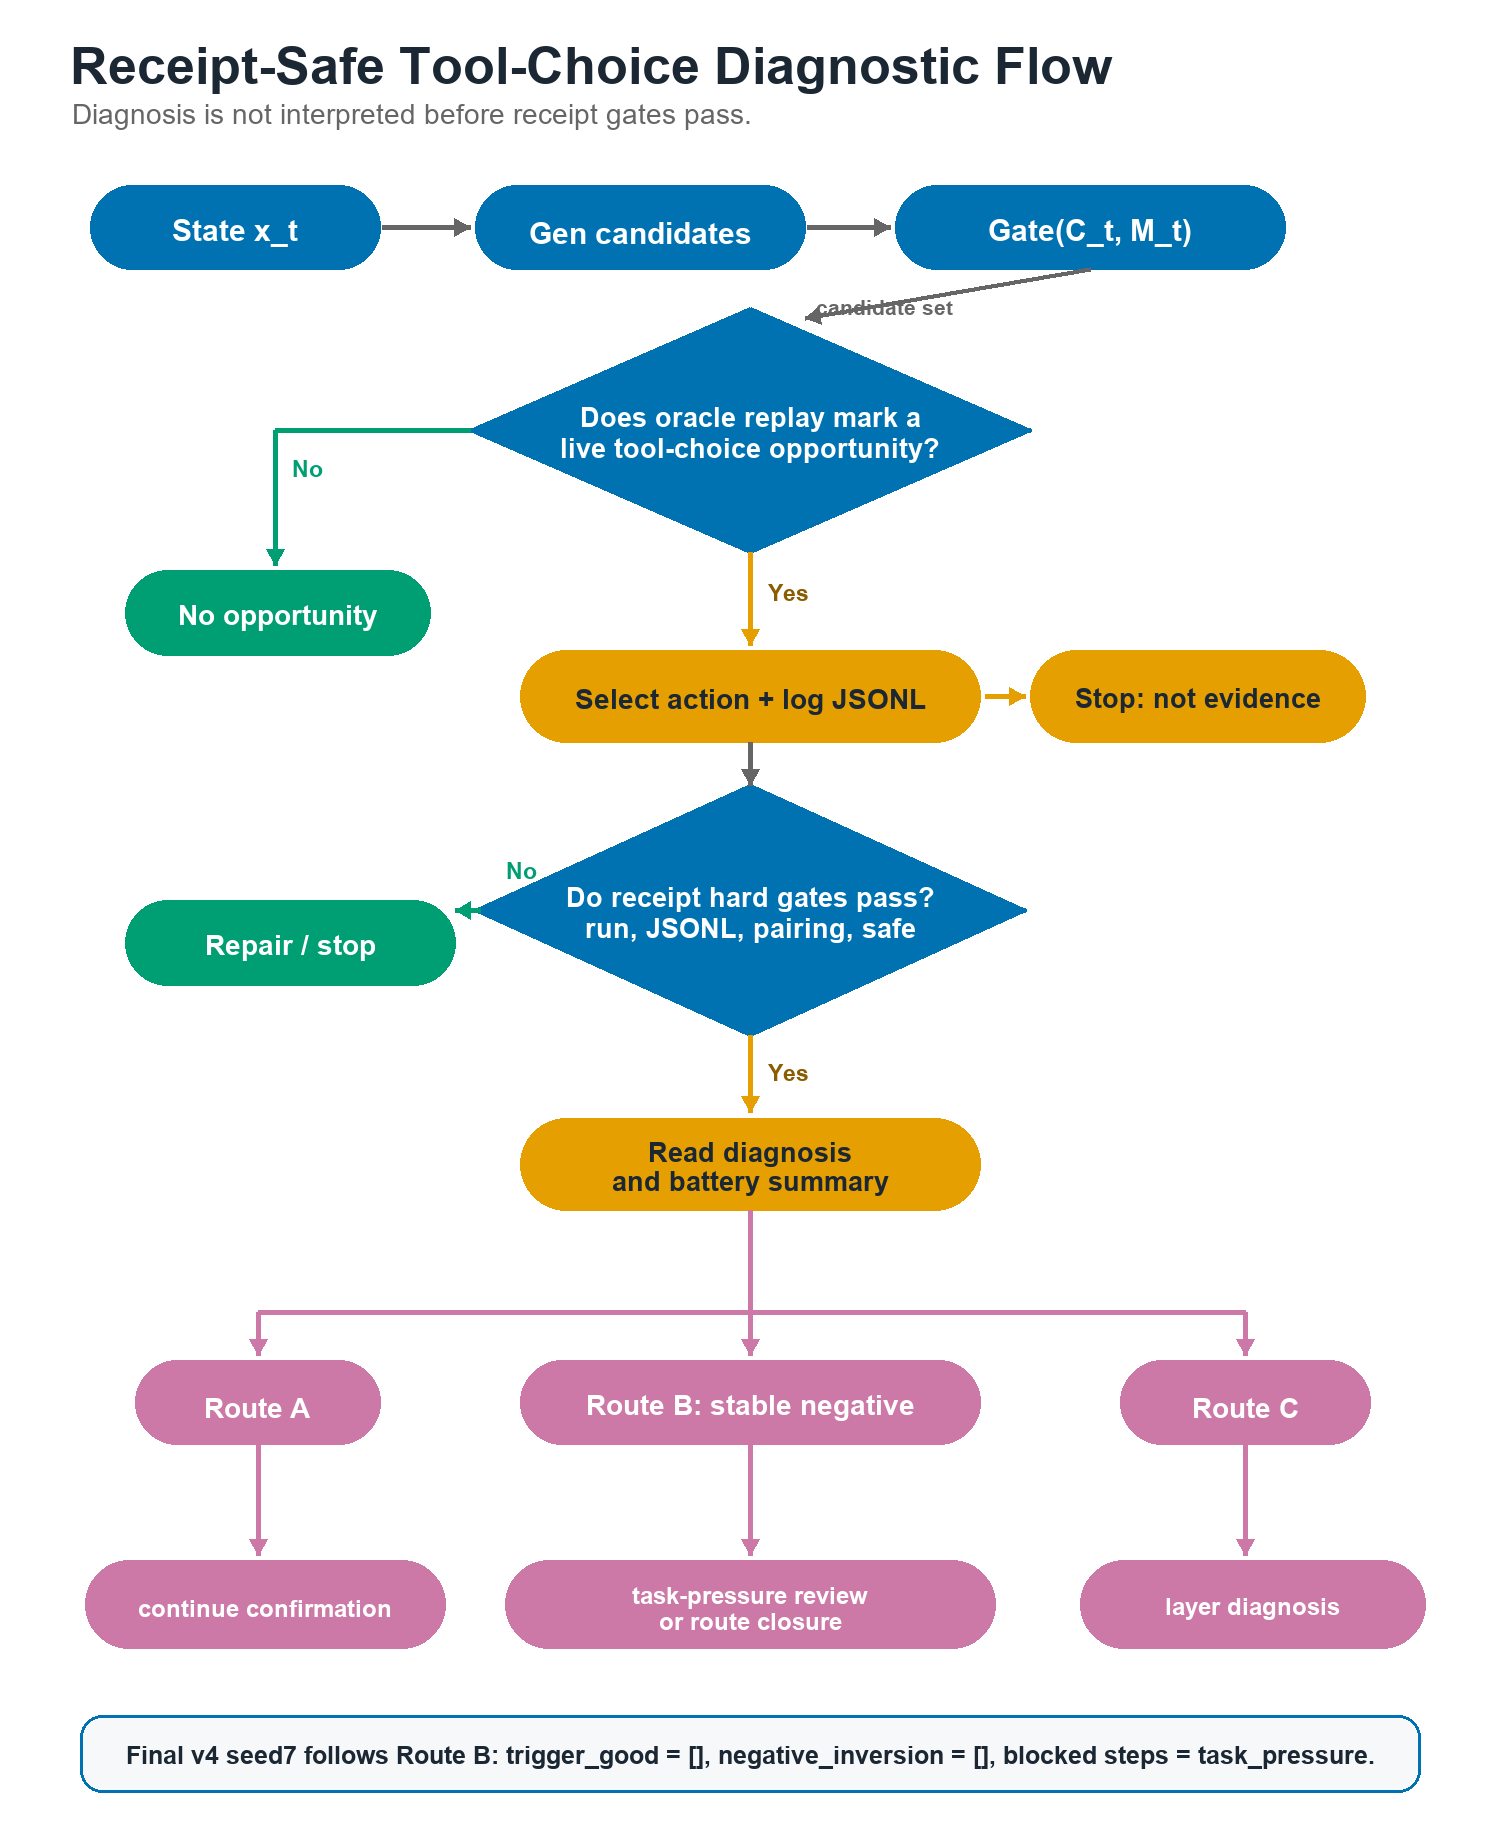
\includegraphics[width=0.70\textwidth]{pipeline_flowchart.png}
\caption{Receipt-gated decision pipeline. The gate is an ask-candidate filter, not the final selector, and diagnosis is interpreted only after the live JSONL passes the receipt hard gates.}
\label{fig:pipeline}
\end{figure*}

\paragraph{Memory and preflight.}
\texttt{voi\_memory\_v1} stores typed \texttt{decision\_lesson} records. Each lesson contains a tool family, local scope, trigger condition, action bias, and provenance. Operationally, retrieval maps a matched lesson to a small score-level bias on family-tagged candidates before selection; it is a VOI-inspired control signal, not a learned estimator of information value. Retrieval is family-scoped: lessons about verify are meant to influence verify-relevant steps rather than all asking behavior. This is intentionally weaker than claiming robust semantic understanding; it tests whether structured textual control signals can become behaviorally consequential, in the spirit of agent-model and verbal-memory work \citep{andreas2022agentmodels,park2023generative,shinn2023reflexion}.

Step-local preflight is an offline guard before live execution. It checks that a generated pack contains successor states where asking has positive value and direct choice does not dominate almost everywhere. This prevents a trivial distribution where all modes look good because the correct behavior is almost always immediate choice.

\paragraph{Receipts and route decisions.}
The receipt layer is a reproducibility check rather than an analysis tool. A run must satisfy \texttt{run\_completed=true}, \texttt{jsonl\_integrity=pass}, \texttt{task\_id\_pairing=pass}, and \texttt{safe\_for\_interpretation=true}. Only then do the diagnosis scripts compare the selected tool family with the oracle family. The route labels are bookkeeping: A means continue confirmation, B means the locked comparison is negative or still dominated by task pressure, and C means negative inversion that would justify inspecting the gate, memory, or selector. The final battery lands in B.

\begin{table}[t]
\footnotesize
\centering
\setlength{\tabcolsep}{3pt}
\begin{tabular}{@{}p{0.33\columnwidth}p{0.61\columnwidth}@{}}
\toprule
Term & Operational meaning \\
\midrule
Tool-choice opportunity & A step where oracle replay exposes a relevant epistemic tool family and multiple tool/choose alternatives are live. \\
Step-local preflight & Offline pack check that asks remain valuable after one-ask successor states, not only at the initial state. \\
\texttt{decision\_lesson} & Typed memory record with family, scope, trigger, action bias, and provenance. \\
Choose-swallow & Rate at which a mode chooses directly despite an oracle tool-choice opportunity. \\
Negative inversion & A harmful case where \texttt{voi\_memory\_v1} is worse than the selector baseline on the stress pack. \\
Blocked-step routing & Diagnosis of blocked \texttt{voi\_memory\_v1} ask opportunities into task pressure, surfaced ask deficit, or hard cutoff. \\
\bottomrule
\end{tabular}
\caption{Key definitions added in response to midway feedback.}
\label{tab:defs}
\end{table}

\section{Experiments}

All experiments use internally generated tasks rather than a public benchmark. This limits external realism but makes attribution tight, unlike broad evaluation suites that emphasize coverage across many tasks or behavioral capabilities \citep{ribeiro2020checklist,bowman2021benchmarking,liang2023helm,srivastava2023bigbench,liu2024agentbench,jimenez2024swebench}. Each live battery compares \texttt{full} (baseline), \texttt{selector\_penalty} (a non-memory anti-ask variant), and \texttt{voi\_memory\_v1} (family-scoped lessons). A battery is interpreted only if both packs pass four receipt gates: run completion, JSONL integrity, task-id pairing, and safety for interpretation.

Table~\ref{tab:ladder} shows the post-midway ladder. The midway report ended at a 10-task smoke batch. The final project adds seed-7 v3 dual-battery evidence, a seed-11 stress-only probe, a repaired seed-11 reference confirmation battery, v4 offline repair, and a v4 seed-7 receipt-safe live battery.

Failed packs are kept out of live evidence. A reference pack that fails combined preflight is not frozen, hashed, or used in a battery summary, and a stress-only separation is not treated as confirmation. This accounting matters for the final result: the negative finding is not based on one weak probe, but on a sequence of receipt-safe comparisons that failed to turn stronger task pressure into a locked memory advantage.

\begin{figure*}[t]
\centering
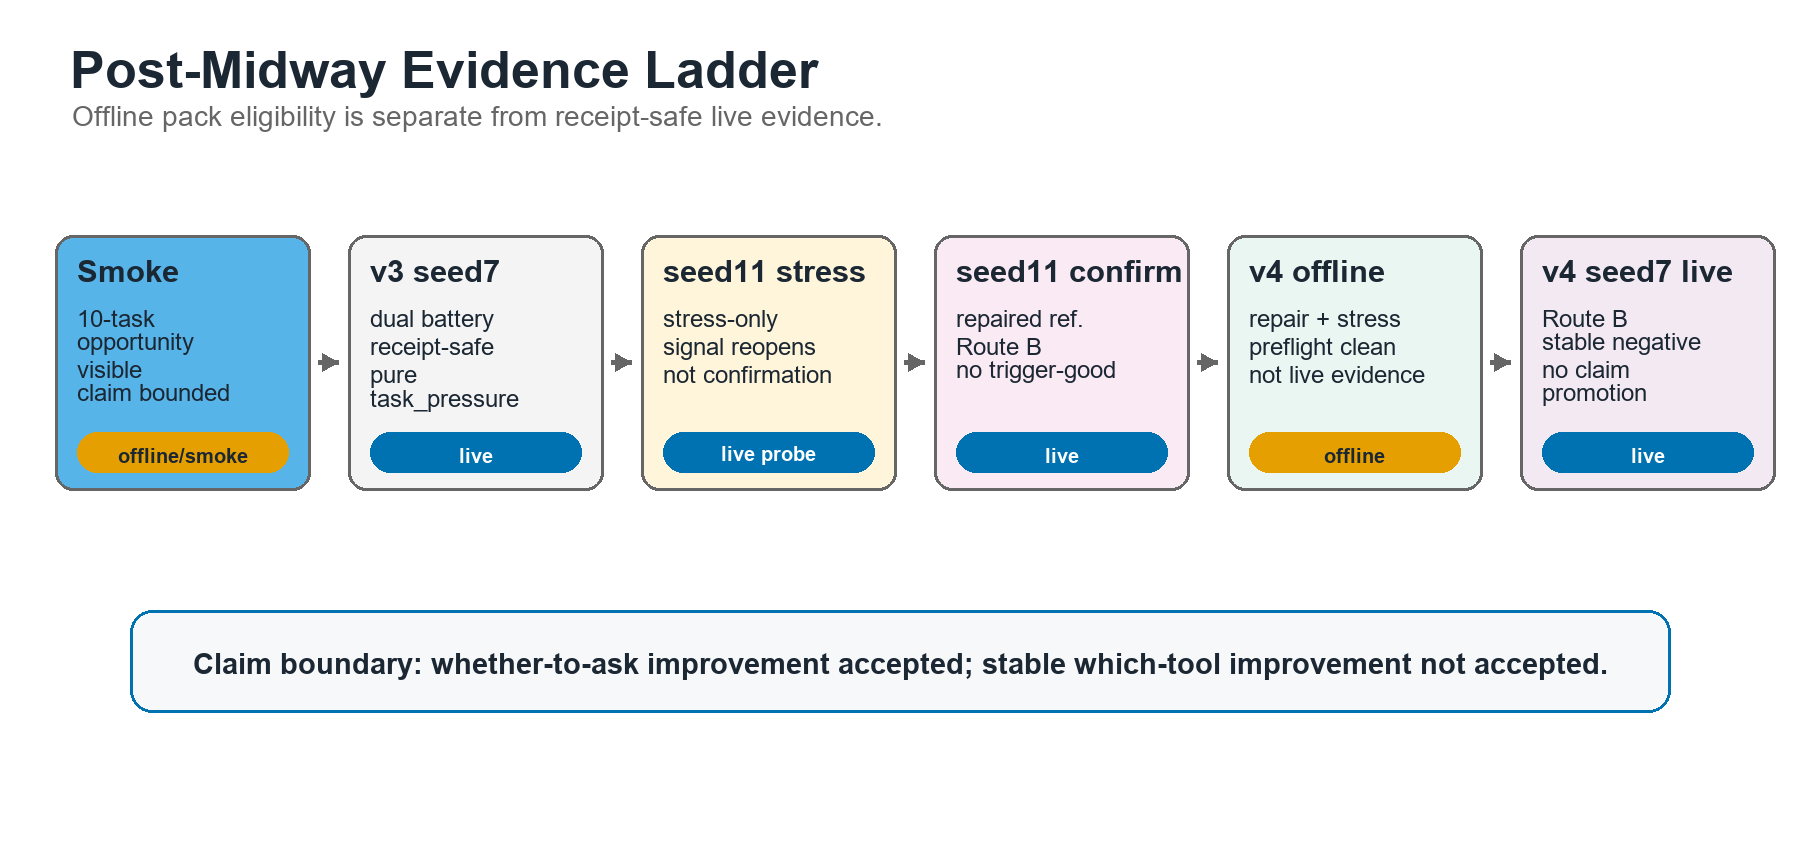
\includegraphics[width=0.96\textwidth]{evidence_ladder.png}
\caption{Post-midway diagnostic ladder. The visual separates offline pack eligibility from receipt-safe live evidence, ending in a Route B stable negative rather than claim promotion.}
\label{fig:ladder}
\end{figure*}

\begin{table*}[t]
\scriptsize
\centering
\setlength{\tabcolsep}{3pt}
\begin{tabular}{@{}p{0.16\textwidth}p{0.15\textwidth}p{0.21\textwidth}p{0.12\textwidth}p{0.25\textwidth}@{}}
\toprule
Stage & Seed/profile & Reference/stress status & Receipt status & Main outcome \\
\midrule
Midway smoke & seed 7, \texttt{verify\_necessary} & 10-task step-local smoke & receipt checked & Nonzero opportunity, no accepted which-tool claim \\
v3 dual battery & seed 7, v3 stress & frozen reference vs v3 stress & both pass & Collapse on locked primary comparison; pure task pressure \\
seed-11 probe & seed 11, v3 stress & stress-only probe & stress pass & Stress-only family-mismatch separation reopens, but not confirmation \\
seed-11 confirmation & seed 11, repaired reference + v3 stress & repaired reference vs existing stress & both pass & Route B; no trigger-good; no negative inversion \\
v4 offline repair & seed 7, v4 stress & reference repair + regenerated stress & offline only & Both packs pass preflight; not live evidence \\
v4 live battery & seed 7, v4 stress & repaired reference vs v4 stress & both pass & Route B; stable task-pressure negative result \\
\bottomrule
\end{tabular}
\caption{Post-midway experimental ladder. Offline diagnostics are kept separate from receipt-safe live evidence.}
\label{tab:ladder}
\end{table*}

\section{Results and Analysis}

The final v4 seed-7 battery is the main evidence. Both reference and stress packs pass the receipt layer. The summary has no trigger-good case for the locked memory mode and no negative inversion; it therefore routes to task-pressure or stable-negative review.

\begin{table*}[t]
\scriptsize
\centering
\setlength{\tabcolsep}{4pt}
\begin{tabular}{@{}llrrrrrrr@{}}
\toprule
Pack & Mode & Tool & Oracle & Cov. & Swallow & Fam. & Verify & Wrong \\
\midrule
\multirow{3}{*}{Ref.} & full & 45 & 145 & .310 & .690 & .690 & .103 & .000 \\
& sel-pen & 10 & 110 & .091 & .909 & .909 & .036 & .000 \\
& voi-mem & 89 & 189 & .471 & .529 & .529 & .206 & .000 \\
\midrule
\multirow{3}{*}{Stress} & full & 51 & 151 & .338 & .662 & .927 & .298 & .000 \\
& sel-pen & 21 & 121 & .174 & .826 & .975 & .174 & .000 \\
& voi-mem & 86 & 186 & .462 & .538 & .538 & .086 & .000 \\
\bottomrule
\end{tabular}
\caption{Final v4 seed-7 battery metrics. Tool and Oracle are selected and oracle tool-choice step counts; Cov. is realized coverage. Swallow and Fam. mismatch are lower-better error rates; Verify is higher-better verify-use rate; Wrong is lower-better wrong-tool rate. The locked \texttt{voi\_memory\_v1} reference-vs-stress comparison does not improve the which-tool metrics.}
\label{tab:final}
\end{table*}

\begin{figure*}[t]
\centering
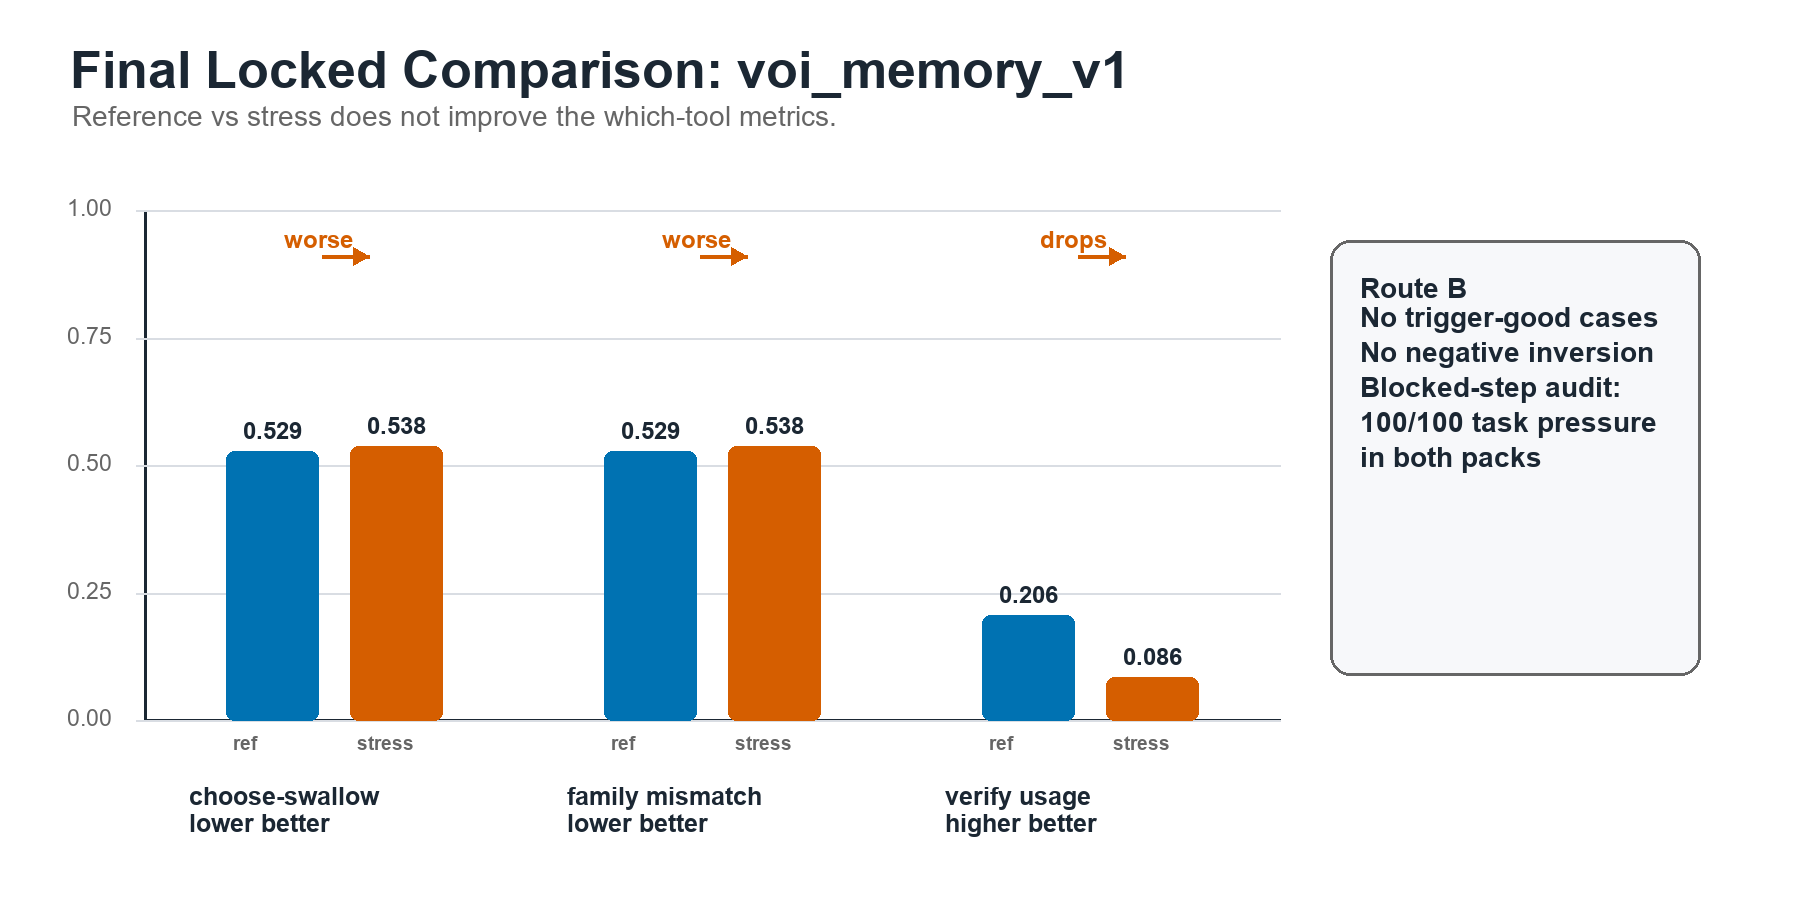
\includegraphics[width=0.90\textwidth]{v4_final_metrics.png}
\caption{Final locked \texttt{voi\_memory\_v1} comparison. Lower is better for choose-swallow and family mismatch, while higher is better for verify usage; the v4 stress pack does not improve the locked which-tool surface.}
\label{fig:metrics}
\end{figure*}

The key row is \texttt{voi\_memory\_v1}. Choose-swallow and selected-vs-oracle family mismatch are both 0.5291 in the reference pack and 0.5376 in the v4 stress pack. Verify usage drops from 0.2063 to 0.0860. The stronger task ecology therefore did not turn memory into a stable which-tool improvement. The policy often reaches tool-choice opportunities, but it still swallows many of them by choosing directly or by failing to use the oracle family.

The stress pack does expose wrong-tool surface in \texttt{full} and \texttt{selector\_penalty}, where family mismatch rises above reference. That confirms that the v4 stress design created sharper scan/verify conflict. In \texttt{voi\_memory\_v1}, however, the surface does not become a verify success; it appears alongside high choose-swallow and lower verify usage.

\begin{figure*}[t]
\centering
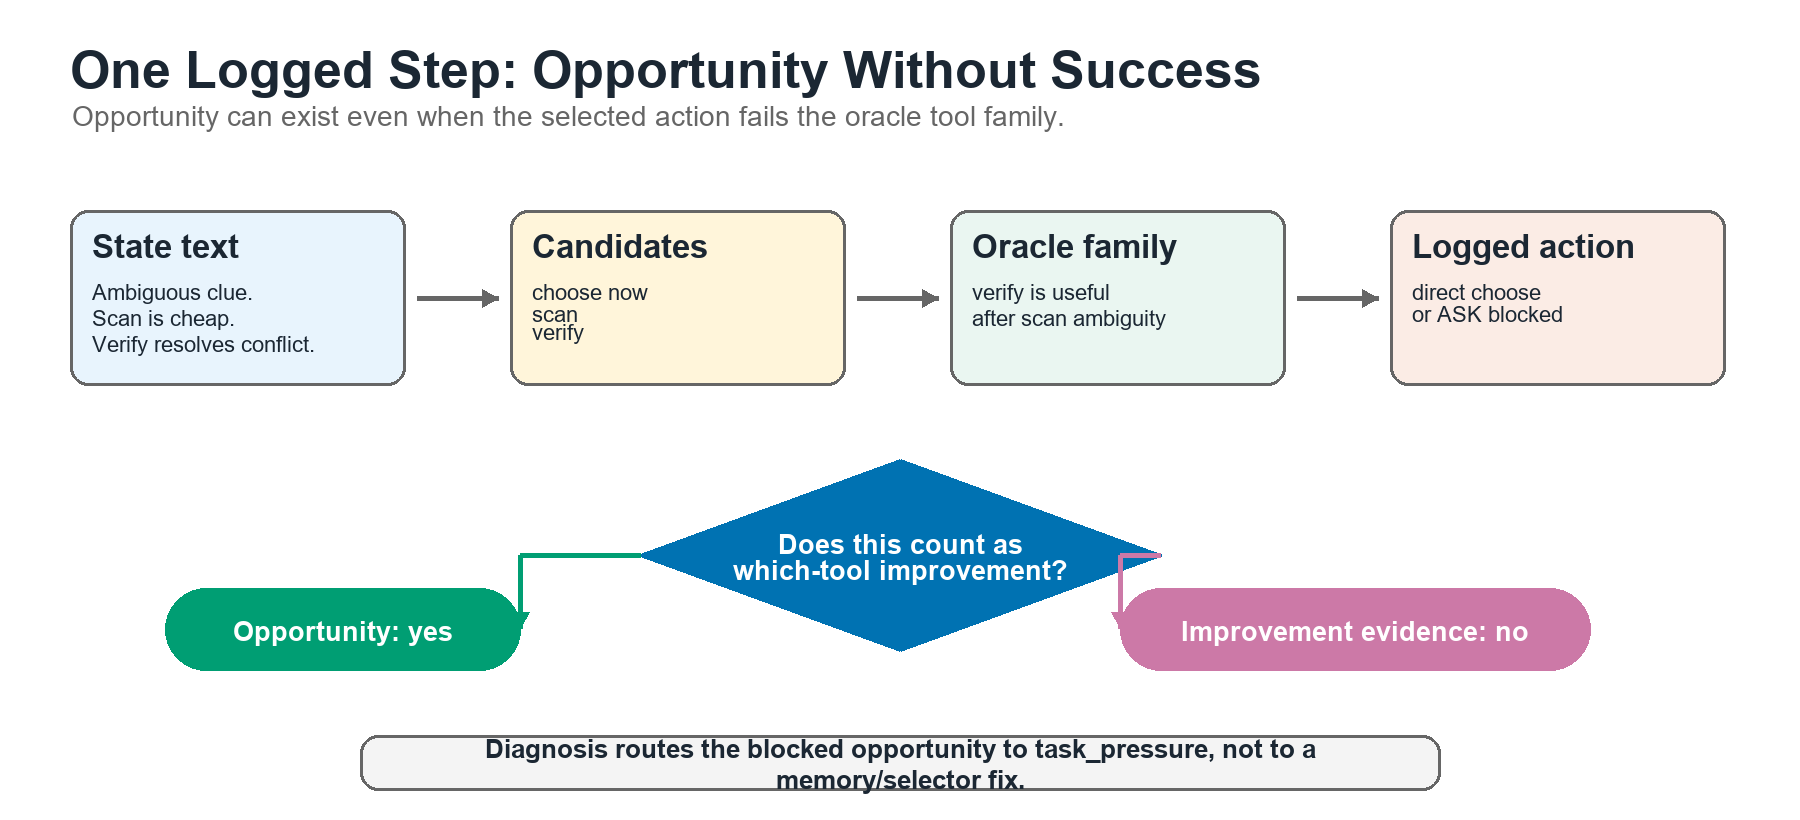
\includegraphics[width=0.90\textwidth]{case_walkthrough.png}
\caption{Case-step visualization. A step can count as a tool-choice opportunity while still failing the locked memory comparison because the selected action does not realize the oracle verify family.}
\label{fig:case}
\end{figure*}

Figure~\ref{fig:case} shows the denominator used in the analysis. It is not all environment steps; it is the subset where oracle replay says a tool family is relevant and the action space still contains meaningful tool/choose alternatives. Within that subset, direct choice is counted as choose-swallow rather than a tool-family success. The accepted conclusion is therefore narrow: \texttt{voi\_memory\_v1} improved whether-to-ask behavior in the earlier single-tool setting, but the final batteries do not establish stable which-tool improvement.

\paragraph{Error anatomy.}
The final failure is not a logging artifact and not simply a lack of task difficulty. The v4 stress pack does expose more wrong-tool surface in the non-memory modes, which means the generator successfully created more scan/verify conflict than the earlier smoke setting. The locked memory mode, however, does not convert that exposed surface into verify usage. Its reference and stress family-mismatch rates remain nearly identical, and the stress-side verify usage falls below the reference side. The mechanism therefore looks like unrealized task pressure: the live policy sees opportunities but still fails to turn them into the oracle family action. This does not prove that the memory code is independently broken; it shows that, in this environment, structured memory bias is too weak or too poorly aligned to overcome direct-choice pressure.

\paragraph{Interpreting the route.}
The route is more specific than saying the experiment ``did not work.'' The run is valid, the JSONL can be interpreted, no negative inversion justifies a layer switch, and the locked primary comparison does not support a positive which-tool claim. This is important because the seed-11 stress-only probe briefly looked encouraging: family mismatch improved inside the stress pack. The repaired seed-11 reference confirmation and the v4 seed-7 live battery prevent that local pattern from being overpromoted.

\paragraph{Why not patch memory or selector now.}
The blocked-step audits route both final packs to \texttt{task\_pressure}: 100 out of 100 blocked rows in the reference pack and 100 out of 100 in the stress pack. There is no surfaced ask deficit and no hard-cutoff candidate share. That does not prove memory and selector design are perfect. It says something narrower: the current receipts do not localize the failure to those layers. A selector or memory patch would be a new hypothesis about how to fight choose-swallow, not a conclusion licensed by this battery.

\section{Discussion and Limitations}

The project is small, and the negative result is local. Its strength is diagnostic control rather than headline performance. The system records when an offline pack is not eligible, when a live run is safe to interpret, and when a stress-only signal is not enough. This emphasis on evaluation protocol follows work arguing that benchmark design, behavioral tests, data-regime choices, and score stability can change conclusions about system quality \citep{ribeiro2020checklist,bowman2021benchmarking,warstadt2023babylm,liang2023helm,levtsov2025confidence}.

The main limitation is external validity. ToyTextMDP is synthetic and far smaller than open-ended code or web environments \citep{chen2021codex,jimenez2024swebench}. Its advantage is exact replay and attribution, but the same control can make the state space pathological. For example, the v4 verify-usage drop could mean that \texttt{voi\_memory\_v1} failed, or that this micro-MDP created pressure where verify and scan are formally distinguishable but not semantically rich enough for a language-memory cue to matter. The safe interpretation is therefore local: receipt-safe negative evidence under this task ecology, not a universal claim that VOI memory cannot help tool choice.

A second limitation is the memory abstraction itself. The \texttt{decision\_lesson} schema is structured text converted into candidate-family score bias. That is useful for a controlled mechanism test, but it is not a deep semantic model of information value. The negative result may therefore challenge the representation assumption as much as the task design. Future work should compare this hand-structured memory against learned value predictors, paraphrase-stable triggers, and family-label swap tests before calling any positive effect semantic VOI reasoning.

The choose-swallow pattern also raises a broader agent-design question. If a policy repeatedly chooses directly despite receipt-safe tool-choice opportunities, natural-language penalties and discrete recalled lessons may be too weak to counter an immediate-generation prior. The present study cannot settle that question, because no negative inversion or surfaced ask deficit justifies a layer switch. It does, however, make the failure observable enough to test stronger anti-swallow designs as new hypotheses rather than retroactive explanations.

This version incorporates the midway feedback by defining the project terms operationally, decomposing the pipeline into generation, gating, selection, receipt, and diagnosis, and separating ``opportunity exists'' from ``which-tool improvement is supported.''

The next scientific step is not to patch the gate or selector immediately. The current evidence points to either closing the present route as a stable negative result, or redesigning task pressure with even more live-aligned oracle exposure. A layer switch should require negative inversion or direct layer evidence, neither of which appears in the final battery.

\section{Conclusion}

Structured memory did not improve the locked which-tool comparison under the current task ecologies. The useful result is the evaluation sequence itself: it exposes tool-choice opportunities, rejects an unsupported positive claim, and points the next review toward task pressure rather than gate, memory, or selector changes.

\section*{Author Contributions}

Bochuan Yao designed and implemented the toolized environment, VOI memory variants, task profiles, live batteries, diagnosis pipeline, and report analysis.

\section*{Code and Artifacts}

The public code and artifact repository is \url{https://github.com/yaobc77-ai/cs505-playground-final-artifacts}.

\bibliography{references}

\end{document}
